% based on the CVPR template provided by Ming-Ming Cheng (https://github.com/MCG-NKU/CVPR_Template)
% modified and extended by Stefan Roth (stefan.roth@NOSPAMtu-darmstadt.de)

\documentclass[10pt,twocolumn,letterpaper]{article}

%%%%%%%%% PAPER TYPE
\usepackage[pagenumbers]{cvpr}

% Include other packages here, before hyperref.
\usepackage{graphicx}
\usepackage{amsmath}
\usepackage{amssymb}
\usepackage{booktabs}

% If you comment hyperref and then uncomment it, you should delete
% Hadley_Proposal.aux before re-running LaTeX.
% (Or just hit 'q' on the first LaTeX run, let it finish, and you
%  should be clear).
\usepackage[pagebackref,breaklinks,colorlinks]{hyperref}

% Support for easy cross-referencing
\usepackage[capitalize]{cleveref}
\crefname{section}{Sec.}{Secs.}
\Crefname{section}{Section}{Sections}
\Crefname{table}{Table}{Tables}
\crefname{table}{Tab.}{Tabs.}

\begin{document}

%%%%%%%%% TITLE
\title{CS 153 Project Proposal\\
Mapping the density of flowers on California buckwheat plants
}

\author{Alex Hadley\\
Harvey Mudd College\\
Claremont, CA\\
{\tt\small ahadley@hmc.edu}
}
\maketitle

% %%%%%%%%% ABSTRACT
% \begin{abstract}
%    The ABSTRACT is to be in fully justified italicized text, at the top of the left-hand column, below the author and affiliation information.
%    Use the word ``Abstract'' as the title, in 12-point Times, boldface type, centered relative to the column, initially capitalized.
%    The abstract is to be in 10-point, single-spaced type.
%    Leave two blank lines after the Abstract, then begin the main text.
%    Look at previous CVPR abstracts to get a feel for style and length.
% \end{abstract}

%%%%%%%%% BODY TEXT
\section{Motivation}

Honey bees and native bumble bees are important pollinators of both agricultural and wild plants~\cite{Potts}. However, recently the populations of both bees have declined. Donkersley \etal~\cite{Donkersley} have shown that landscape composition is important to the nutrition of honey bees, and Donaldson-Matasci and Dornhaus~\cite{Donaldson} have shown that species richness and flower density are important variable affecting honey bee communication. Examing these factors invovles mapping out the locations of flowers; however, current methods of doing so are either too labor-intensive (\eg ground-based surveys) or lack detail (\eg satellite imaging).

Professor Donaldson-Matasci's Bee Lab at Harvey Mudd College is using high-resolution drone imaging, which provides more detail than satellite imaging but scales more easily than ground surveys. So far, the lab has been able to classify plants by species and generate bounding polygons (see Figure~\ref{fig:annotation}). The next step in their pipline is to identify the density of flowers on these plants. Initially, the lab is interested in the plant \textit{Eriogonum fasciculatum}, the California buckwheat, but they hope to extend flower detection to other plants in the future. The ability to generate detailed maps of flowers and compare them to the nutritional status of bees will help develop models predicting the affects of land use and climate change on pollinators.

\begin{figure}[t]
  \centering
   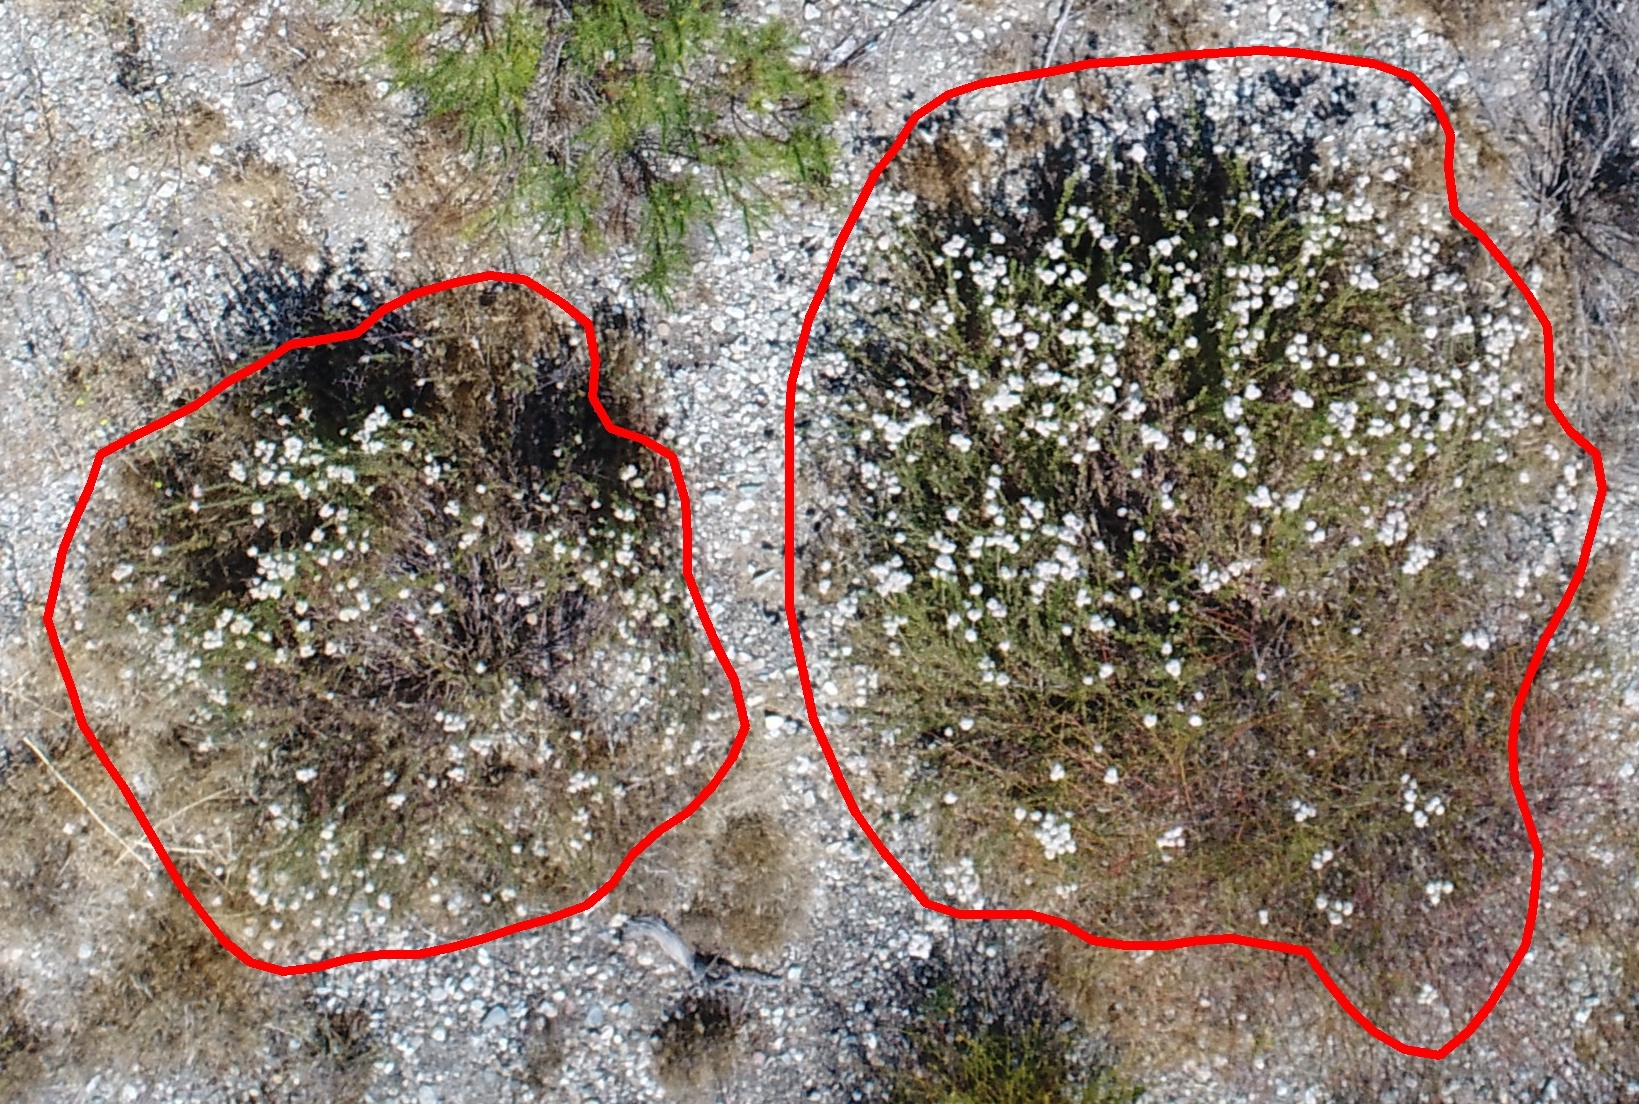
\includegraphics[width=0.9\linewidth]{annotation.jpg}
   \caption{An example of a polygon annotation outlining a California buckwheat plant.}
   \label{fig:annotation}
\end{figure}

\section{Methods}

The goal of this project is, given a drone image and a bounding polygon (see Figure~\ref{fig:annotation}), to return the total number of pixels within the polygon, the number of those pixels corresponding to flowers, and a mask of the flower pixels.

The provided data includes images with corresponding JSON files containing lists of plants in the image, along with a bounding polygon for each. Code to plot these polygons has been provided by Tom Fu.\footnote{\url{https://github.com/tommyfuu/flower_map_new/blob/master/scripts/visualizePolygons.py}} The next step will be to convert the polygons into binary masks in order to count the total number of pixels in the plant regions, and to isolate the plant regions for flower identification. This will be done using OpenCV's \texttt{fillPoly} function.\footnote{\url{https://docs.opencv.org/3.4/d6/d6e/group__imgproc__draw.html}}

The task of labeling pixels in an image according to categories is known as semantic segmentation. A classical method of accomplishing this is color thresholding, which involves tuning lower and upper limits in the RGB or HSV color spaces and labeling pixels within the limits as flowers. Although this method is relatively easy to implement, it does not perform well since threshold values are sensitive to particular lighting conditions and do not take morphological features into account~\cite{Dias}. I intend to use color thresholding as a baseline model; however, I expect the model to incorrectly label the white rocks seen in Figure~\ref{fig:annotation} or have trouble working well in different lighting, such as in Figure~\ref{fig:annotation2}.

\begin{figure}[t]
  \centering
   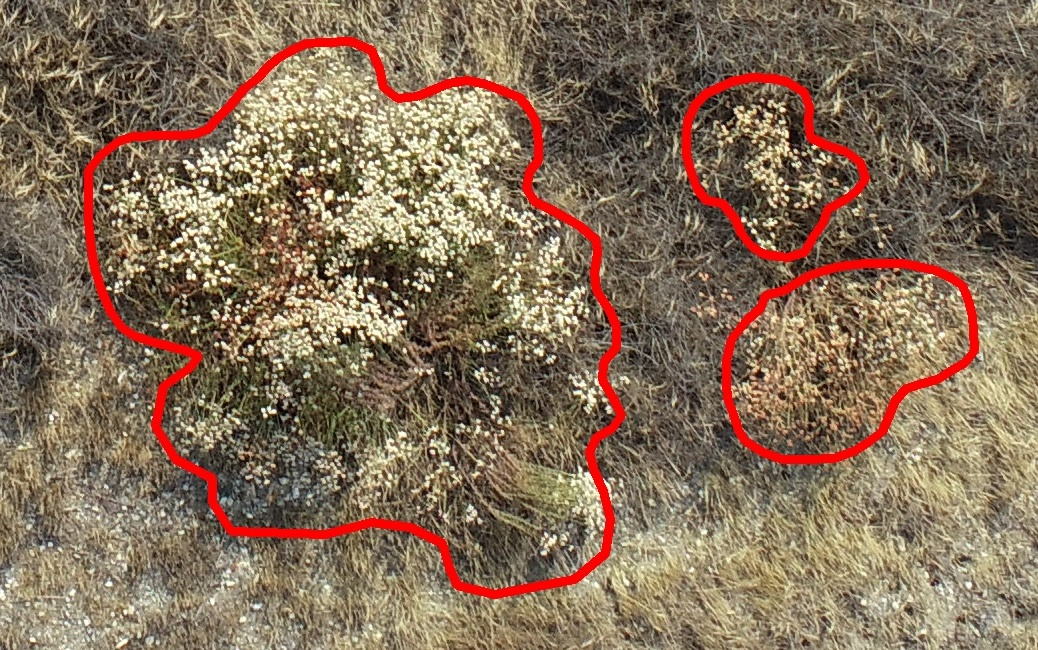
\includegraphics[width=0.9\linewidth]{annotation2.jpg}
   \caption{An example California buckwheat plants in different lighting than Figure~\ref{fig:annotation}.}
   \label{fig:annotation2}
\end{figure}

A more promising method involves using a convolutional neural network (CNN). A well-known model that combines semantic segmentation with object detection is Mask R-CNN~\cite{He}, and it has been used to identify plant features, such as by Machefer \etal~\cite{Machefer}. However, use cases for Mask R-CNN typically involve distinguishing individual objects, which is not one of the goals for this project.

One semantic segmentation model that only labels pixels rather than detecting objects is SegNet~\cite{Segnet}. SegNet has been used by Palacios \etal~\cite{Palacios} for identifying grapevine flowers. Using the SegNet architecture with a VGG19 network as the encoder, they were able to achieve an F1 score of $0.930 \pm 3.15\%$ for their segmentation task.

Another promising model used by Dias \etal~\cite{Dias} is DeepLab~\cite{Deeplab}. Like SegNet, DeepLab labels pixels according to different categories, which Dias \etal use to detect fruit flowers, achieving F1 scores between 74\% and 86\% across several species, which greatly outperformed their HSV-based baseline model.

After creating a baseline model based on HSV thresholding, I intend to use either SegNet or DeepLab to increase performance. Dias \etal also divide their images into smaller ``portraits'' and passing those through their CNN~\cite{Dias}. Given that the plant regions in this project have varying sizes, I think this would be a promising method to use. Since the flowers are already small, I do not want to resize the images, so cropping seems like the best option. Furthermore, detecting flowers in one region of the plant should not depend on features from other regions, meaning that examining subregions independently should work well.

Given a plant region, I will take a bounding rectangle and divide this into squares. The squares will have some overlap in order to account for the potential of features' being underweighted near the edges. I plan to train and run the CNN on these subregions, and then take a union of the resulting masks to create an overall flower mask for the plant. Finally, I will discard flower pixels outside of the plant's bounding polygon.

In order to train the model (either SegNet or DeepLab), I plan to use PyTorch and implement a similar method to Dias \etal~\cite{Dias}, which invovles using weights pre-trained on the COCO-Stuff dataset and fine-tuning the model to recognize the specific flowers in question. This dataset already includes labels for common features such as flowers and grass, so the pre-trained model should be a good starting point.

In order to train and test the model, I will require the data to be annotated with pixels corresponding to flowers. I will then divide the regions and annotations into square subregions as described above, and use those as input to the CNN.

\section{Measuring success}

I plan to measure success quantitatively based on precision, recall, and F1 scores of the proportion of correctly predicted pixels within the plant regions. I will also qualitatively measure the success of the models by comparing the output flower masks to the ground truth annotations. I will also compare the performance of the CNN model to the baseline HSV model to ensure that the extra computation is worth it.

\section{Challenges}

One challenge is that the plant regions are not square or even rectangular and are not consistently sized, so they cannot be passed directly into a CNN. I plan to address this using the method described above, where I take a bounding rectangle of the region and divide it into partially overlapping squares, using the squares as independent input to the CNN. This also has the advantage of not needing to rescale the images, which potentially loses important detail for small flowers.

Another challenge lies in annotating the data. There are 888 images containing 11,981 plants. It will be a challenge to annotate enough plants to train and test a model well. There is no need to annotate all of the data, but it is important to aquire enough sample data to train on. One solution will be to share the work of annotation with other CS 153 students working on this project. It will also be important to sample images from the different batches provided in order to produce a robust model, since they were taken in different regions and in different lighting conditions.

Another challenge will be actually training these CNN models since I do not have much experience doing so. A solution will be examing how this is done in the papers, reading PyTorch tutorials online, and getting help from Professor Wloka or other students working on the project. Also, I have identified two potential models, SegNet and DeepLab, so that if I have trouble implementing one, I will hopefully be able to use the other.

\section*{Acknowledgements}

I discussed this project with Thuy-Linh Le, another CS 153 student working on this project.

%%%%%%%%% REFERENCES
{\small
\bibliographystyle{ieee_fullname}
\bibliography{egbib}
}

\end{document}
